
\chapter{使用技术}

本章阐述本研究的整体设计。整体设计部分在基本原理之上,给出更具体的实现方案设计。从本研究的目标出发,为了提供可以运行于FPGA SoC平台的深度学习框架,首先应确定用什么FPGA SoC平台和使用什么样的开发工具。其次,如果自行从头构建深度学习框架,一方面工作量过于庞大、需要考虑很多优化问题;另一方面也缺乏足够的受众,研究人员更熟悉流行的深度学习框架。因此应选用成熟的流行的深度学习框架作为基础,在其上进行针对特定嵌入式平台的适配与优化。

基于上述的考虑,本章首先介绍Xilinx Zynq平台的系统架构、搭载的ARM与FPGA的硬件特点、以及本研究使用的基于Zynq的开发板Zedboard的具体特性等等。之后给出Xilinx SDSoC工具的基本情况介绍,包括其包含的工具以及支持的开发流程。随后介绍本研究选用的基础深度学习框架Caffe,主要涉及与后续开发密切相关的软件架构和实现方式。最后,综述整体设计方案,即本研究的最终结果是如何有机结合ZYNQ,SDSoC和Caffe。

\section{Zynq平台}

Zynq平台的全称是“全可编程SoC”(All Programmable SoC),由双核的ARM Cortex-A9处理系统(Processing System,简称PS)与Xilinx可编程逻辑(Programmable Logic,简称PL)组成。除此以外,还包含片上内存(On-chip memory),外部内存接口(External Memory Interface),各类外围设备输入输出接口(I/O Peripherals and Interfaces)以及连接PS与PL的高速AXI总线等等。

本研究基于Zynq平台的最新系列Zynq-7000进行系统设计与实现。

\subsection{Zynq系统架构}

Zynq平台的系统架构如图2.1所示。接下来分块介绍Zynq的几个组成部分。

\begin{figure}[!ht]
\centering
	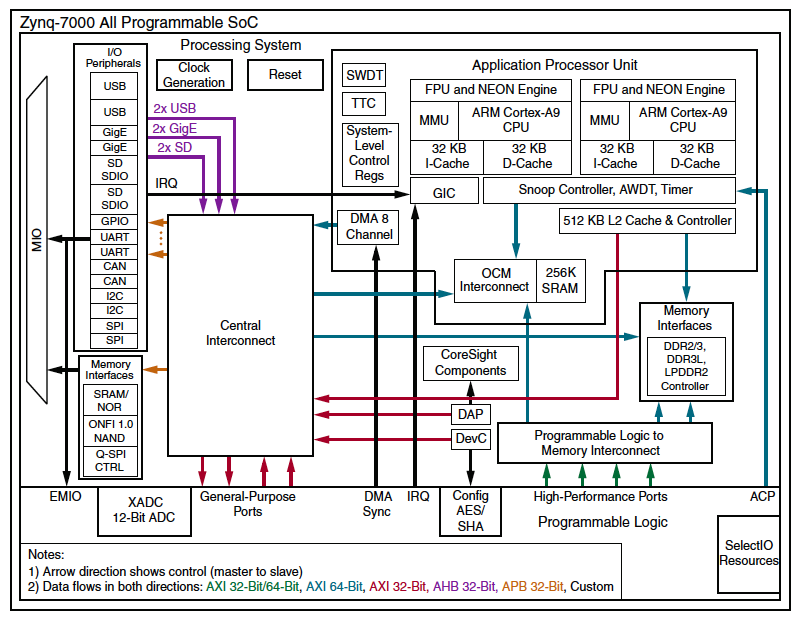
\includegraphics[width=0.8\textwidth]{assets/imgs/zynq-7000}
\caption{Zynq-7000平台的系统架构}
\end{figure}

\subsubsection{ARM处理系统}

Zynq SoC系统上搭载了双核ARM Cortex-A9 MPCore处理器,该处理器可以运行到最高1GHz,拥有指令和数据的32KB L1缓存与512KB L2缓存,以及NEON媒体处理引擎(media-processing engine)和浮点数向量处理单元(Vector Floating Point Unit,简称VFPU)等等。Cortex-A9的性能十分优异,足以满足多种情况下的计算需求。

本研究中依赖该ARM处理器提供的CPU端环境进行大部分的计算。有关ARM处理器与内存系统和PL的交互接口在2.1.4节介绍。

\subsubsection{可编程逻辑}

Zynq的可编程逻辑(PL)与一般的FPGA设计一致,主要包含CLB,BRAM以及DSP处理单元。相关指标如下表所示:

\begin{table}[!ht]
\begin{tabular}{ | p {3cm} | l | l | l | l | }
\hline
Programmable Logic Cells & LUTs & Flip-Flops & BRAMs & DSP Slices \\ \hline
85K & 53,200 & 106,400 & 560 KB & 220 \\
\hline
\end{tabular}
\caption{Zynq-7000 XC7Z020可编程逻辑上资源容量}
\end{table}

本研究使用的XC7Z020系列Zynq的可编程逻辑的配置与性能大致上与Artix-7 FPGA相似,硬件资源比较有限。因此想要取得高效的性能必须做精细的资源分配和优化。相关的优化策略和技巧在第四章详述。

\subsubsection{数据通路AXI与存储系统}

存储系统与数据通路负责连接处理系统与可编程逻辑,以及处理和其他外围设备通信。Zynq平台的存储系统主要由三个部分组成:处理系统中的缓存(L1与L2 cache)和片上内存(On-chip Memory);可编程逻辑上的BRAM;以及大容量的外部存储(External Memory)。Zynq上的几种数据通路可以完成这三个组成部分之间的不同形式的交互。

Zynq上的数据通路的基础是ARM的AXI(Advanced eXtensible Interface)总线协议,属于AMBA(Advanced Microcontroller Bus Architecture)协议的一部分。AXI的最新版本是AXI4协议,Xilinx设计并实现了基于AXI4的IP核,使得AXI变得更加灵活、高效和便捷。AXI4协议主要有三类:针对大数据量传输的AXI4,小数据量的AXI4-Lite,以及针对流数据的AXI4-Stream。Zynq上的数据通路正是基于Xilinx提供的AXI IP核实现的。

Zynq基于AXI总线协议连接处理系统和可编程逻辑,主要实现两类接口:高性能AXI端口(High-Performance AXI ports)与ACP(Accelerator Coherency Port)接口,二者区别关键在内存数据一致性上。高性能AXI端口可以实现处理系统和可编程逻辑高速的数据传输,但不保证CPU缓存中的数据与内存读写一致。ACP接口则在硬件机制上保证缓存中的数据在传输之前被写回内存、内存更新之后缓存同步更新。

在设计Zynq应用时具体使用哪种数据通路取决于系统的特性。本研究在第三章给出对数据通路选择的原则,在第四章会具体讨论两种数据通路的性能对比。

\subsection{Linux运行模式}
基于Zynq平台开发的应用有两种运行模式:Standalone与Linux模式。前者代表应用的运行不用启动操作系统,后者则要求先启动Linux操作系统再运行应用。考虑到深度学习应用并不是简单的计算,还需要各种数据处理的操作,并且科研人员更熟悉基于操作系统的运行模式,本研究只在Linux模式下进行开发。

Linux模式首先启动预先加载与ROM中的引导程序,该程序从SD卡中读取第一阶段启动程序(First Stage Boot Loader, 简称FSBL),FSBL负责处理可编程逻辑的比特流(bitstream)和Linux引导程序(u-boot)的加载与执行。引导程序之后分别加载Linux的镜像文件(uImage)、设备树文件(Device Tree)和根系统文件(Rootfs)。Linux镜像主要包含Linux内核,设备树文件定义了硬件设备环境供引导程序动态加载,根系统文件则包含了系统的根目录和必要的程序与库。准备就绪之后即可通过UART接口或者SSH连接到Zynq平台,运行程序或进行开发。

Xilinx提供了bootgen工具来创建SD卡引导程序,以及一系列预生成的文件,例如Linux镜像,根系统文件等等。SDSoC工具中包含了bootgen,以及更多跟硬件平台相关的预生成文件,可以更简便地生成SD卡中需要的内容。在2.3节中会进一步介绍。

\subsection{Zedboard}
本研究选用的是Zedboard作为Zynq开发平台。Zedboard是基于Zynq-7000系列的扩展式处理平台,Zedboard上除了满足Zynq-7000所要求的ARM Cortex-A9 MPCore处理器与Xilinx FPGA之外,还增加了如下配置:512MB DDR3内存、256MB QSPI闪存和一系列输入输出接口(HDMI、VGA、OLED与音频接口)等等。除此以外,Zedboard成本低廉,还有Xilinx SDSoC的特别支持,尤其是预先搭载好的输入输出接口对深度学习应用的开发(计算机视觉等应用)非常方便。因此本研究使用Zedboard作为最终深度学习框架所运行的平台。

\section{SDSoC开发环境}

Xilinx于2015年3月推出了SDSoC开发环境,提供类似于嵌入式C/C++开发体验。SD即“软件定义”(Software Defined):SDSoC的目标是降低FPGA应用开发门槛,让更多的软件开发者,而不是专业的FPGA开发人员,可以通过C/C++代码直接生成Zynq SoC系统。此外,SDSoC综合了Vivado HLS,Xilinx ARM GNU编译工具链,以及一系列系统生成工具(bootgen, Xillybus等等),令开发效率得到很大提升。但是SDSoC的最大优势在于其对传统SoC开发流程的改进。接下来主要介绍SDSoC的开发流程与基本使用方式。

\begin{figure}[!ht]
\centering
	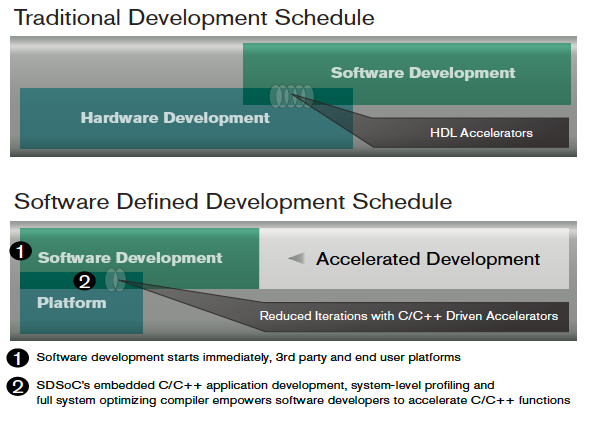
\includegraphics[width=0.7\textwidth]{assets/imgs/software-defined}
\caption{传统的开发流程(Traditional Development Schedule)与软件定义的开发流程(Software Defined Development Schedule)的区别}
\end{figure}

\subsection{软件定义的开发流程}

传统的SoC平台的系统开发流程首先需要完成硬件部分的设计,之后软件开发者才能通过已经综合实现好的硬件接口进行进一步开发。这种开发流程迭代周期非常长,软件部分的开发在硬件设计过程中处于停滞状态,硬件设计只能等软件部分完成才能获得反馈。基于SDSoC的开发基于软件定义的开发流程:先用C/C++代码完成整个系统的设计,之后以函数为单元部署于可编程逻辑,进行硬件加速。SDSoC甚至提供了硬件加速性能预测工具,可以令开发人员在长时间的综合实现完成之前就能大概了解目前的优化策略是否正确。图2.2是对两种开发流程的对比。

\subsection{基本概念与使用方式}

\subsubsection{数据移动网络}
SDSoC开发环境关键概念是数据移动网络(data motion network),表示PS与PL之间的数据通路模式:SDSoC使用预先设计好的数据通路IP核来负责PS与PL之间的数据传输,这些IP核称为数据移动单元(data mover)。比如AXIDMA\_SG就表示通过AXI总线用Scatter-Getter的方式通过DMA传输数据。数据移动单元与数据类型密切相关,标量数据只能用AXI\_LITE传输,而数组与更复杂的数据类型可以用AXI\_DMA\_SG,AXI\_DMA\_SIMPLE,AXI\_DMA\_2D等数据传输单元传输。一般而言SDSoC可以根据数据类型,内存分配方式等分析出最适合使用的数据传输单元,但开发者也可以使用预编译指令(pragma)进行优化。

\begin{figure}[!ht]
\centering
	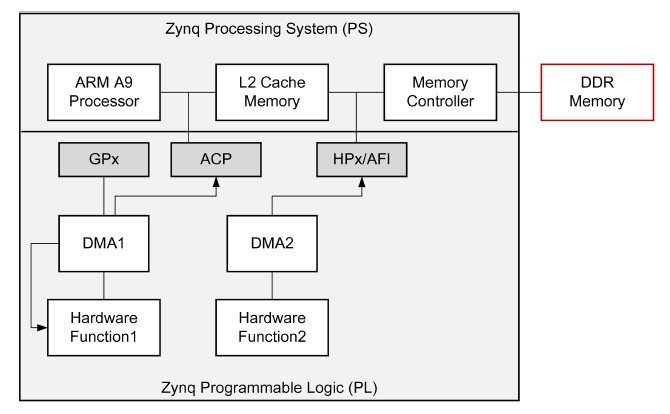
\includegraphics[width=0.8\textwidth]{assets/imgs/zynq-axi}
\caption{Zynq AXI总线协议的几种端口}
\end{figure}

\subsubsection{使用方式}
SDSoC的可以通过其IDE使用,也可以基于纯粹的Linux命令行使用。由于IDE的限制更多,本研究完全使用命令行环境开发。SDSoC的最关键工具是sdscc/sds++。这两个程序本质上为C/C++编译器,可以完全兼容gcc/g++的命令行选项。但与一般编译器不同,sdscc/sds++可以通过命令行选项指定:1)需要HLS的函数:包含函数名和要求的时钟频率;2)数据移动网络的时钟频率;3)目标硬件平台:比如zed(针对Zedboard)或zybo(针对ZYBO开发板)。因此,通过sdscc/sds++工具可以轻易与原有的Linux项目进行兼容。有时候也需要更细粒度的操作,可以使用arm-xilinx-linux-gnueabi的GNU工具链对C/C++代码进行交叉编译,使用sdslib封装IP核等等,在第三章对Caffe和第三方库的移植中会详细介绍。

本研究的应用完全依赖SDSoC进行开发,利用Vivado HLS进行硬件逻辑编写和优化,SDSoC自带的IP核进行数据通路的自动生成,以及Xilinx ARM GNU工具链编译CPU端代码并进行链接。最后SDSoC把项目全部整合到SD卡中。

\section{深度学习框架Caffe}

Caffe\supercite{jia2014caffe}是加州伯克利大学计算机视觉与学习中心\footnote{Berkeley Vision and Learning Center,\url{http://bvlc.eecs.berkeley.edu/}}开发的深度学习框架,基于C++与CUDA开发。Caffe因其速度快,数据模版清晰易懂,并拥有开源的、高度模块化的代码而广受开发者欢迎。

本研究选用Caffe作为移植到Zynq上进行移植和加速的对象,主要是因为其清晰的软件架构,非常便于修改和优化。除此以外,与其他深度学习框架(如基于LuaJIT的Torch,基于Python的Theano)相比,Caffe的CPU端代码完全基于C++实现,与高层次综合工具、ARM GNU编译工具链、SDSoC等等可以无缝衔接。因此本研究最终选用Caffe作为优化的基础。

接下来首先介绍Caffe的使用中出现的关键概念,之后着重介绍与移植相关的Caffe软件架构和神经网络层的实现。

\subsection{基本概念}
Caffe中的网络层Layer和网络Net是两个关键概念。Caffe Layer是对神经网络层的抽象,通过指定使用的预定义网络类型,上下层连接的网络名称,以及本层的参数就可以构建一个Caffe Layer。Caffe Layer之间连接起来的有向无环图(Directed Acyclic Graph,简称DAG)便是Caffe Net,即神经网络。Caffe的神经网络训练是用Caffe Solver(求解器)实现的,一个Caffe Solver中定义了训练的网络名称、控制训练的参数以及运行的硬件(CPU或GPU)等等。Caffe Layer、Caffe Net和Caffe Solver都可以使用Google Protocol Buffer\footnote{Google Protocol Buffer (\url{https://developers.google.com/protocol-buffers/docs/overview})不仅提供了一种接口数据传输的格式,同时还可以生成数据传输与序列化的代码。}文档格式进行定义。

从具体实现的角度出发,理解Caffe的代码关键需要理解Layer类和Blob类。每个Caffe的Layer类都实现了Forward与Backward两个方法,相当于神经网络中的前向与反向计算。Forward与Backward的两个参数都是用Blob类表示的网络层输入输出。Blob类本质上是多维数组,因此可以处理各种形状的网络层输入输出。

Caffe的标准用法有两种,一种是通过编译出的caffe命令行工具直接训练Caffe模型,其中Caffe模型与训练数据需要提前定义好;除此以外,也可以使用Caffe动态链接库(libcaffe.so)在其他的C++应用中使用Caffe提供的接口。两种方法都十分方便。

\subsection{软件架构}
% 这一部分之后需要进一步扩充,主要是面向对象设计的部分:Blob类是什么,Net和Layer类是什么等等
Caffe的软件架构主要包含如下几个部分,依赖关系具有清晰的分层次的结构:
\begin{enumerate}
\item 基础架构:数据类型的定义,比如blob.cpp定义了Blob数据结构,net.cpp与layer.cpp分别定义了网络类与网络层类。同时常用数学函数math\_functions.cpp也十分重要,Caffe的各种大运算量的计算基本都会调用该文件所定义的函数。
\item 网络层的实现:在layers/目录下定义了常见的神经网络层的实现,比如卷积神经网络conv\_layer.cpp,ReLU层relu\_layer.cpp等等。相关GPU代码也包含其中。
\item 求解器实现:在solvers/目录下定义了多种求解器。
\item 其他:比如Caffe使用的Protobuf文件等等。
\end{enumerate}

\subsection{第三方库依赖}
Caffe所依赖的第三方库不多,可以简单分为如下几类:
\begin{enumerate}
\item 数据存储:LMDB与LevelDB
\item 数据格式和接口:HDF5与Protobuf
\item 数学计算:BLAS库比如ATLAS或OpenBLAS
\item 其他:比如日志Google glog,基础组件Boost 等等
\end{enumerate}

总之,Caffe的分层设计和简单的第三方库依赖都非常便于优化和修改。本研究针对Caffe的移植与优化在第三章中详述。

\section{综合设计方案}


